
\documentclass[10pt]{beamer}
\usepackage{kotex}

\usepackage{framed}
\usepackage{graphicx}
%https://www.overleaf.com/learn/latex/Inserting_Images

\usepackage{amsmath}
%use dfrac
\usepackage{xcolor}

\usepackage{amsthm}
%\usepackage{tabl}
\usepackage{listings}
\definecolor{mGreen}{rgb}{0,0.6,0}
\definecolor{mGray}{rgb}{0.5,0.5,0.5}
\definecolor{mPurple}{rgb}{0.58,0,0.82}
\definecolor{backgroundColour}{rgb}{0.95,0.95,0.92}
%https://tex.stackexchange.com/questions/348651/c-code-to-add-in-the-document
\lstdefinestyle{CStyle}{
    backgroundcolor=\color{backgroundColour},   
    commentstyle=\color{mGreen},
    keywordstyle=\color{magenta},
    numberstyle=\tiny\color{mGray},
    stringstyle=\color{mPurple},
    basicstyle=\footnotesize,
    breakatwhitespace=false,         
    breaklines=true,                 
    captionpos=b,                    
    keepspaces=true,                 
    numbers=left,                    
    numbersep=5pt,                  
    showspaces=false,                
    showstringspaces=false,
    showtabs=false,                  
    tabsize=2,
    language=C
}

\usepackage{url}

\usepackage{etoolbox}
\AtBeginEnvironment{quote}{\singlespacing\small}


\usepackage{thmtools}
\usepackage{xcolor}
\declaretheoremstyle[% spaceabove=6pt,spacebelow=6pt, headfont=\color{MainColorOne}\sffamily\bfseries, notefont=\mdseries, notebraces={[}{]}, bodyfont=\normalfont,
headpunct={},
postheadspace=1em,
%qed=▣,
]{maintheorem}

\declaretheorem[%
name=정의,
style=maintheorem,
numberwithin=section, shaded={%bgcolor=MainColorThree!20,
margin=.5em}]{dfn}
% \begin{dfn}[]
% \end{dfn}

\setbeamertemplate{footline}[frame number]

\usetheme{Hannover}


\title{template / linker}

\author{EUnS}

\begin{document}

%linker
% #include이해
%template
% TMP맛보기
% 과제 3-2

\begin{frame}{}
    \maketitle
\end{frame}    

\begin{frame}{}
    \tableofcontents
\end{frame}   

\section{linker}

\begin{frame}
    \begin{itemize}
        \item 서적 : CSAPP (7장 linker)
        \item 아마 시프시간에 배우는 것.
    \end{itemize}
\end{frame}

\begin{frame}{Complier}
    \begin{figure}[h!]
        \centering
        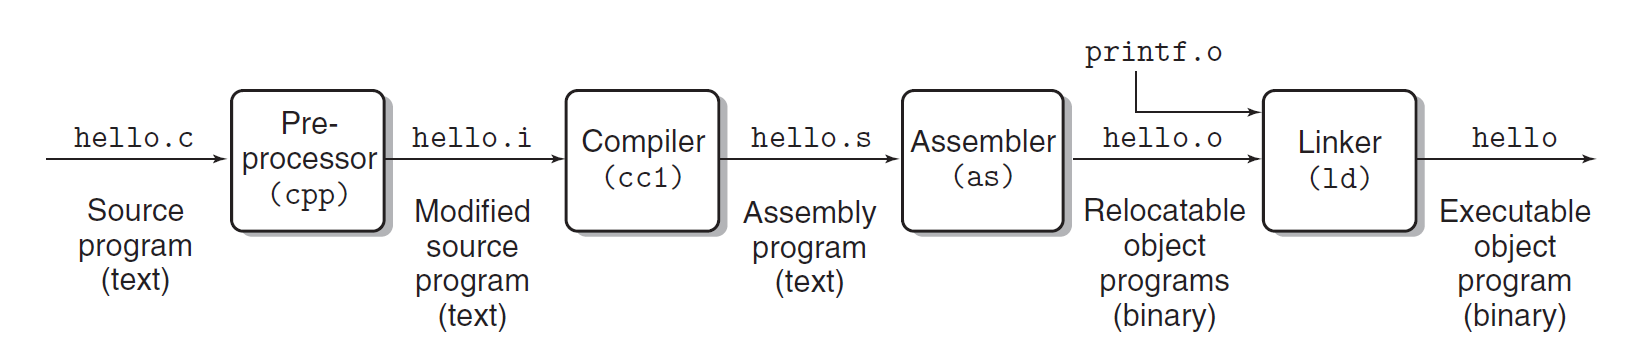
\includegraphics[scale=0.25]{pic1}
        \caption{컴파일 과정}
    \end{figure}
\end{frame}    

\subsection{Object File}
\begin{frame}{Object File}
    
    \begin{itemize}
        \item Relocatable ob~ : compiler,assembler output
        \item Executable ob~ : linker output
        \item shared ob~ : DLL을 위한 파일 생략
    \end{itemize}
\end{frame}    

\begin{frame}{}
    x86-linux : object구조로 ELF(Executable and Linkable Format)사용
    \begin{figure}[h!]
        \centering
        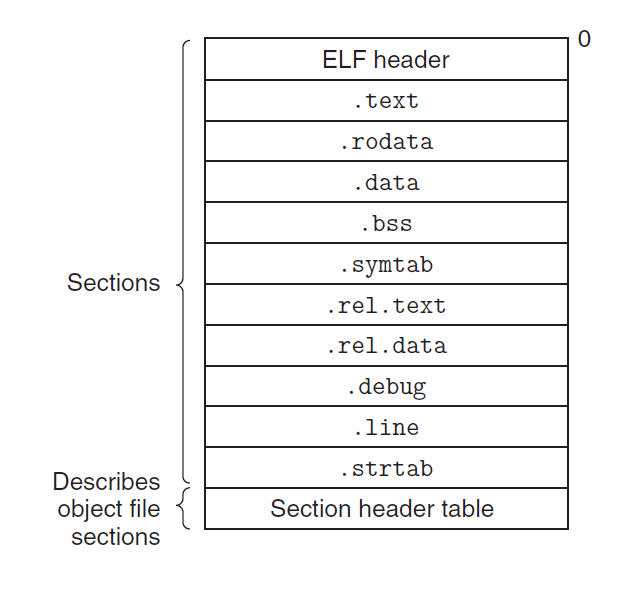
\includegraphics[scale=0.5]{pic2}
        \caption{Typical ELF relocatable object file.}
    \end{figure}
\end{frame}    


%%%%%%%%%%%%%%%%%%%%%%%%%%%%%%%%%%%%%%%%%%%%%%%%%%%%%%%%%%%%%%%%%%
\begin{frame}{}
    \begin{itemize}
        \item \textbf{.text} The machine code of the compiled program.
        
        \item \textbf{.rodata} Read-only data such as the format strings in printf statements, and jump tables for switch statements.
        
        \item  \textbf{.data} Initialized global and static C variables. 
        
        \item \textbf{.bss} Uninitialized global and static C variables, along with any global or static variables that are initialized to zero. block satrted by symbol 의 약어
        
        \item \textbf{.symtab} A symbol table with information about functions and global variables that are defined and referenced in the program. 
    
        \item \textbf{.rel.text} A list of locations in the .text section that will need to be modified when the linker combines this object file with others. 
        
        \item \textbf{.rel.data} Relocation information for any global variables that are referenced or defined by the module.
        
        \item \textbf{.debug} A debugging symbol table with entries for local variables and typedefs defined in the program, global variables defined and referenced in the program, and the original C source file.
        
        \item \textbf{.line} A mapping between line numbers in the original C source program and machine code instructions in the .text section.
        
        \item \textbf{.strtab} A string table for the symbol tables in the .symtab and .debug sections and for the section names in the section headers.
        
    \end{itemize}
\end{frame}    

\subsection{symbol}
\begin{frame}{symbol}
    \begin{itemize}
        \item Global symbols : 모듈 m에 정의되거나 다른 모듈에 참조될 수 있는 심볼 / 전역변수와 static이아닌 함수
        \item Global symbols : 다른 모듈에 정의된 전역변수 
        /다른곳에 정의된 (extern)전역변수와 static이아닌 함수
        \item Local symbols : static으로 선언된 함수, static 전역변수
    \end{itemize}
\end{frame}

\begin{frame}
    Q : 지역 변수는요?

    A : 런타임에 스택에 쌓습니다.
\end{frame}


\subsection{linker}
\begin{frame}{linker 단계}
    \begin{enumerate}
        \item symbol resolution
        \item Relocation
    \end{enumerate}
\end{frame}    


\begin{frame}{Symbol Resolution}
    \begin{itemize}
        \item strong symbol : 초기화된 전역변수, 함수
        \item weak symbol : 초기화x 전역변수
    \end{itemize}
    Rule
    \begin{enumerate}
        \item Multiple strong symbols with the same name are not allowed.
        \item Given a strong symbol and multiple weak symbols with the same name, choose the strong symbol.
        \item Given multiple weak symbols with the same name, choose any of the weak symbols.
    \end{enumerate}
\end{frame}    

\begin{frame}{Relocation}
    \begin{enumerate}
        \item Relocating sections and symbol definitionss :  여러개의 .data section을 합친다.
        \item Relocating symbol references within sections. :모든 심볼 참조를 수정한다. 이후  
        모든 심볼들이 런타임 메모리 주소를 가진다. 어셈블러가 만든 .rel.data section에 있는 Relocation Entries자료구조를 가지고 수행한다
        \begin{itemize}
            \item R\_X86\_64\_PC32 : 상대주소
            \item R\_X86\_64\_32. : 절대주소
        \end{itemize}
         이후 인스트럭션과 전역변수들이 런타임 메모리 주소를 가진다.
    \end{enumerate}
\end{frame} 

\subsection{Executable Object Files}

\begin{frame}{Executable Object Files}
    \begin{figure}[h!]
        %\centering
        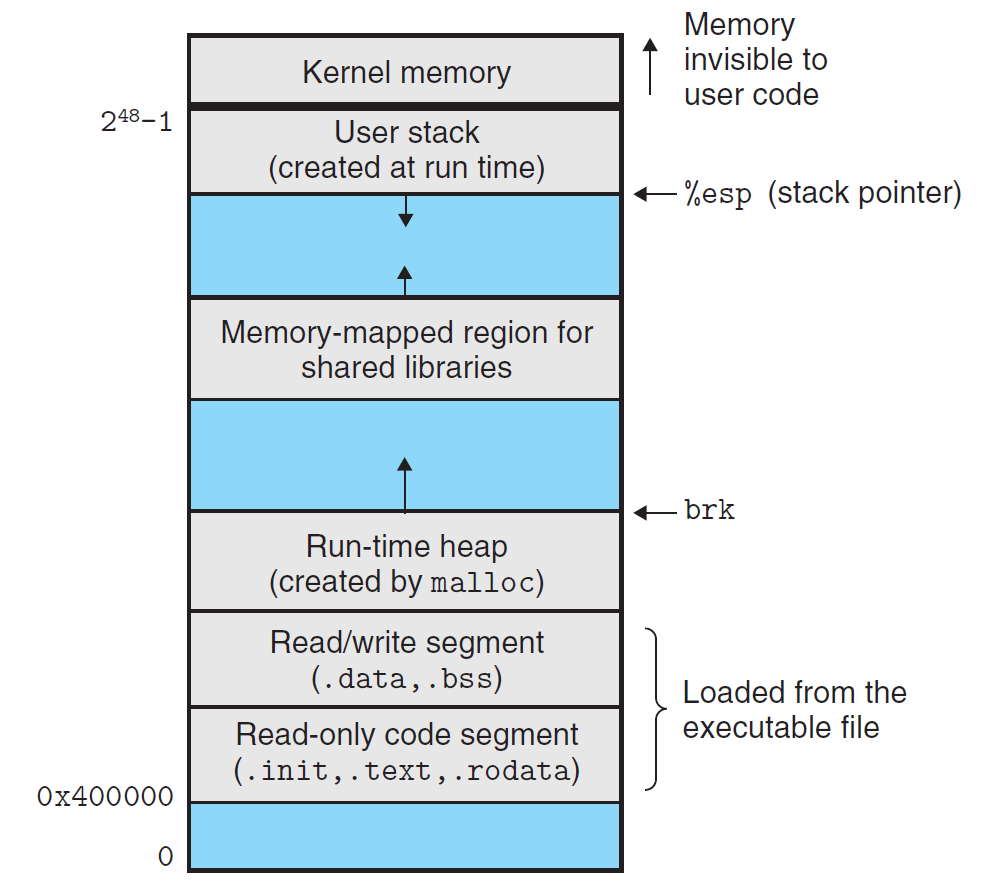
\includegraphics[scale=0.25]{pic4}
        \caption{Typical ELF executable object file.}
    \end{figure}
\end{frame}    

\begin{frame}{Loading}    
    \begin{figure}[h!]
        \centering
        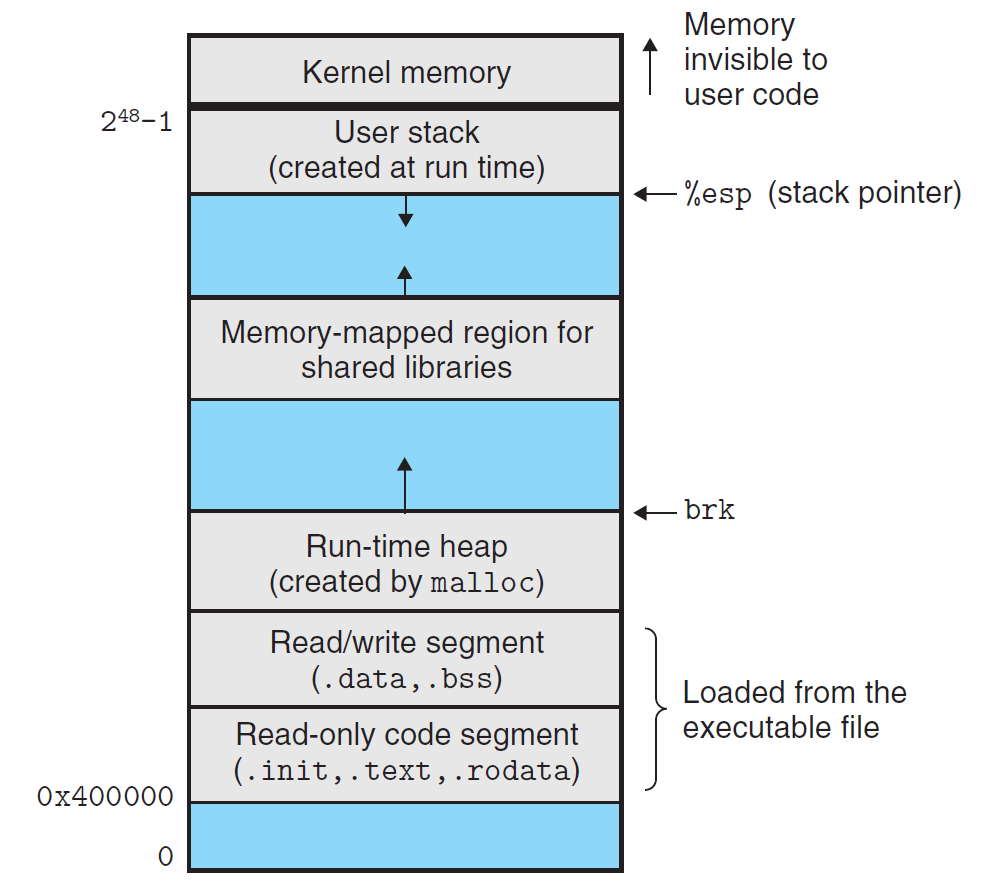
\includegraphics[scale=0.3]{pic5}
        \caption{\textbf{Linux x86-64 run-time memory image.}}
    \end{figure}
    loading : 실행가능한 목적파일 내의 코드와 데이터를 메모리로 복사하고 첫번째 인스트럭션(엔트리 포인트)으로 점프해서실행하는 과정
\end{frame}    

\section{$\#include$이해}

\begin{frame}[fragile]{header file}
    \begin{itemize}
        \item 그냥 텍스트파일과 같다.
        \item 선언을 위한것...
        \item 실제 구현은 어느 cpp파일에서...
        \item $\#include$는 전처리 지시자.
        \item $\#include$로 cpp파일에 그대로 붙여넣는다.
    \end{itemize}
\end{frame}

\section{template}

\begin{frame}{template}
    \begin{itemize}
        \item template을 실제로 인자를 넣어서 사용할때 전처리에서 인자를 넣은 코드를 생성함
        \item 타입 아무거나 넣어도 가능
        \item 실행 파일크기가 예상과 다르게 커질수있음
    \end{itemize}
\end{frame}    


\begin{frame}[fragile]{}
    \begin{lstlisting}[style = CStyle]
        template<typename T>
        T function(T a , T* b, T& c)
        {;}
        template<>
        char function<char>(char a , char* b, char &c)
        {;}

        int main()
        {
            function(1,0x0000,3);
            function("s", 0x0000,"asdf");
        }
    \end{lstlisting}
\end{frame}    



\begin{frame}{}

\end{frame}    

\begin{frame}{}
\end{frame}    

\begin{frame}{}
\end{frame}    

\begin{frame}{}
\end{frame}    


\section{TMP}

\begin{frame}[fragile]{TMP}
    \begin{lstlisting}[style = CStyle]
    template <int N>
    struct Factorial {
        static const int result = N * Factorial<N - 1>::result;
    };

    template <>
    struct Factorial<1> {
        static const int result = 1;
    };
    Factorial<4>::result
    \end{lstlisting}
    \begin{itemize}
        \item template의 특성을 이용해서 반복되는 계산을 컴파일타임에 계산을 해놓은다음 그 값을 $O(1)$에 부르는 흑마법
        \item \href{https://libsora.so/posts/friday-the-13th-tmp/}{\textcolor{blue}{이런짓도 가능}}
    \end{itemize}
    
\end{frame}    

\begin{frame}{TMP는 나쁘다}
    \href{https://www.youtube.com/watch?v=a6BQphLoTag&feature=youtu.be}{\textcolor{blue}{참고}}
    \begin{itemize}
        \item 극암의 코드 가독성
        \item 헬 디버깅
        \item 어려움
        \item 써보고 직접 판단 내려보자.
    \end{itemize}
\end{frame}    


\section{constexpr(c++11)}

\begin{frame}[fragile]{constexpr}
    \begin{itemize}
        \item 변수에 사용할때
        \begin{itemize}
            \item $\#define$ 대체가능
            \item const 상수 대체가능
            \item 컴파일타임에 상수로 대체
        \end{itemize}
        \item 함수에 사용할때
        \begin{itemize}
            \item 어느부분 TMP 대체가능
            \item 컴파일타임에 계산할수도있고 안할수도있음
        \end{itemize}
    \end{itemize}
\end{frame}    

% constexpr code ex 
\begin{frame}[fragile]{}
        
    \begin{lstlisting}[style = CStyle]
    
    \end{lstlisting}

\end{frame}   



% 과제 3-2



\begin{frame}{과제}
    과제 3-2 : 링크드리스트
\end{frame}    


\end{document}


% \begin{frame}{}
% \end{frame}    
%   \href{https://www.youtube.com/watch?v=OMiEwfmfdng&feature=youtu.be}{\textcolor{blue}
\begin{frame}[fragile]{}
        
    \begin{lstlisting}[style = CStyle]
    
    \end{lstlisting}

\end{frame}    
